\documentclass[tikz,border=3.14mm]{standalone}
\usepackage{pgfplots}
\pgfplotsset{compat=1.17}

\begin{document}

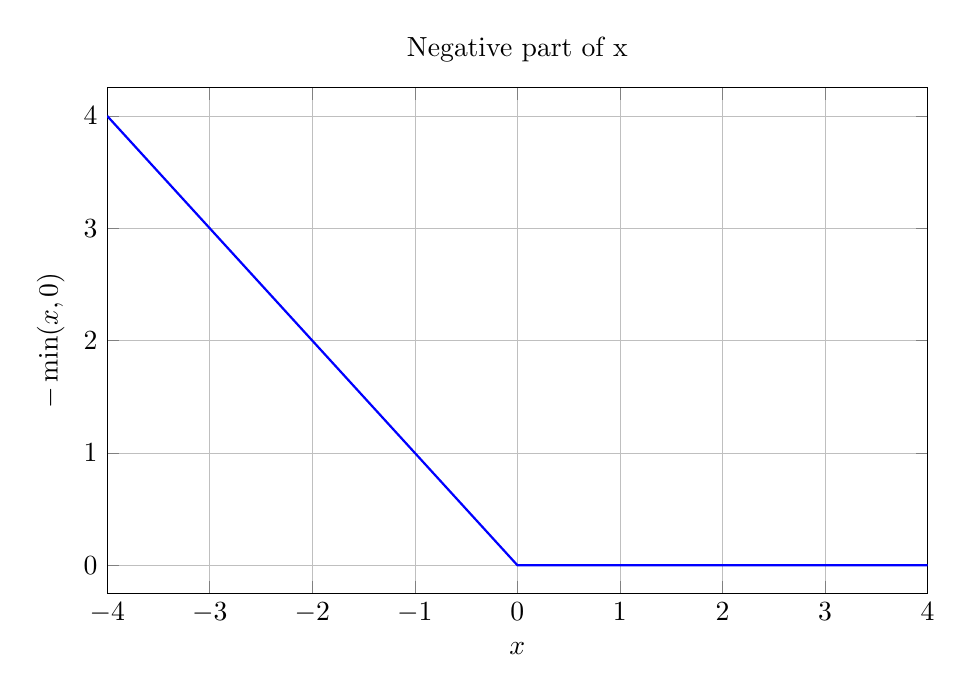
\begin{tikzpicture}
    \begin{axis}[
        xlabel = \(x\),
        ylabel = {\(-\min(x,0)\)},
        domain = -.4:4,
        xmax = 4,
        xmin = -4,
        ymin = -0.25,
        ymax = 4.25,
        samples = 100,
        title = {Negative part of x},
        width = 12cm,
        height = 8cm,
    grid=both,
    grid style={line width=.1pt, draw=gray!10},
    major grid style={line width=.2pt,draw=gray!50},
    ]
    
    \addplot[blue, thick, no markers] (-4,4) -- (0,0) -- (4, 0);
    
    \end{axis}
\end{tikzpicture}

\end{document}
